\documentclass[onecolumn,nocopyrightspace,preprint]{sigplanconf}

\usepackage{booktabs}
\usepackage{listings}
\usepackage{hyperref}
\usepackage{xspace}
\usepackage{caption}
\usepackage[tocentry]{vhistory}
\usepackage{graphicx}
\usepackage{natbib}

% \lstset{
%   commentstyle=\small\ttfamily, %
%   fontadjust=true, %
%   firstnum  ber=1, %
%   escapeinside={(*}{*)}, %
% }

\lstset{
  float=*,
  numbers=none,
  numberstyle=\footnotesize,
  numbersep=4pt,
  basicstyle=\small\ttfamily,
  keywordstyle=\small\ttfamily\bf,
  tabsize=2,
  breaklines=true,
  frame=lines,
  aboveskip=\bigskipamount,
  belowskip=\bigskipamount,
  %belowcaptionskip=\medskipamount,
  language=bash,
  deletekeywords={env, for}
}

\nocaptionrule



\title{Antescofo: Project Title}
\authorinfo{
  Martin~Aigner
}{Computational Systems Group\\University of Salzburg}{firstname.lastname@cs.uni-salzburg.at}

\begin{document}
\maketitle
%\tableofcontents

\section{Foreword} 
Writing this report is part of the requirements of [CLASSNAME] intended to
make students think about combining different topics of education through
a single common property: the use of computers.


Say here, that this is important because...

The goal is to propose a hypothetical project. (to learn this and that)

The cool thing here: this project has actually happened. The drawback: it is no longer a hypothetical project
and therefore, kind of, contradicts the goal of thinking about: ``How would I plan and lead that project?''
Nevertheless, we did plan the project in advance as much as possible and clearly state any changes we have applied 
to \textit{the plan} during the project. Still, we have improvised a lot, e.g., making up on-demand mini lectures on the fly.
The interested reader might wonder if improvisation further contradicts the idea of planning and describing a hypothetical project. 
We don't think so! A teachers ability to adapt to individual student's knowledge, needs, and interests is, in our opinion,
a key quality to have in the educational business.

Our goal with this report is simple. We want to enable others to repeat the project under similar circumstances.
The students achieved a great result which can be viewed at \url{https://youtu.be/a_AVsBpvBVo}

\section{Abstract} 

(Context) The Computational Systems Group Salzburg is involved in a research
project on Antescofo, a real-time multimedia system, developed by IRCAM,
Paris. Antescofo is a complex piece of software used to accompany musicians
and orchestras on the stage. It is used at various concert halls throughout
the world, including the Festspielhaus in Salzburg. We have recently submitted
a research proposal with IRCAM on advancing the real-time aspects of Antescofo
for embedded devices.

(Internship) The task of the students within this internship is to setup, use,
(and so performance analysis of Antescofo. Some of the challenges of Antescofo
(are scalability, as well as proper modelling of time, topics that our
(research group has expertise on. The students are expected to get Antescofo
(running in a lab environment, demonstrate simple use with an actual
(instrument, and isolate performance issues that motivate our research). This
(internship project will be a valuable kick-off for our research on enhancing
(the real-time aspects of Antescofo.

(technical bla-bla) Assets for the students: experience working on a highly
(sophisticated software system; get acquainted with technical issues of
(setting up a system; experience with performance analysis and with research
(on real-time aspects of computing; fun with music and complex software.



\section{Project Goals}


Motivate the students to learn something about the topis needed for the project.

Did you do anything related already? What? How? Any Problems? Anything you want to know?
How can it be useful for you?
What were your motives?

From that we hope to cause an initial motivation of the students. During the class we did THIS AND THAT
to keep them motivated.


Combine computer science, art, and music.


Making music with computers.

The initial goal of the project was evaluating real-time constraints of
Antescofo. However, in an early stage of preparing the project it became clear
that this goal was way too challenging for high-school students without the
required background in real-time systems. Therefore, we changed the scope from
a technical evaluation of the software to an exploration of its artistic
capabilities. We set a new objective: Having fun in the creative process of
making music with computers.


Present your work! Since \textit{video killed the radio star} we will do a music video
that wraps up our project.



\section{Tools}
%Pure Data, Antescofo, Logic, iMovie
This section gives a high level introduction to the software products
used in this projects.

\subsection{Pure Data}

``Pure Data (aka Pd) is an open source visual programming language. Pd enables
musicians, visual artists, performers, researchers, and developers to create
software graphically, without writing lines of code. Pd is used to process
and generate sound, video, 2D/3D graphics, and interface sensors, input
devices, and MIDI. Pd can easily work over local and remote networks to
integrate wearable technology, motor systems, lighting rigs, and other
equipment. Pd is suitable for learning basic multimedia processing and
visual programming methods as well as for realizing complex systems for
large-scale projects.''~\cite{website:puredata}


\subsection{Antescofo}

``Antescofo is a modular polyphonic Score Following system as well as a
Synchronous Programming language for musical composition. The module allows
for automatic recognition of music score position and tempo from a realtime
audio Stream coming from performer(s), making it possible to synchronize an
instrumental performance with computer realized elements. The synchronous
language within Antescofo allows flexible writing of time and interaction in
computer music.''~\cite{website:antescofo}

\subsection{Logic}

\subsection{iMovie}


\section{Tasks}

This section describes the tasks we assign to the students.


\subsection{Setting the project goals}

We decided to let the studets decide on their own what music they wanted to use for the project.
c.f. Hubwieser: Entscheidungssituationen schaffen


\subsection{Setting up the team}

Making the students getting to know each other. First Task: ``Talk about music!''

\subsection{Getting started with Pure Data}

%using the help browser. add screen shot. give example

Antescofo is implemented in - and controlled through - Pure Data.
Installing Pure Data is as simple as installing any OSX application. Details can be found
on the Pure Data website and are not repeated here\footnote{https://puredata.info/downloads}.

A Pure Data application is called a patch. A patch has a graphical Pure Data window



\begin{figure}[ht]
    \centering
    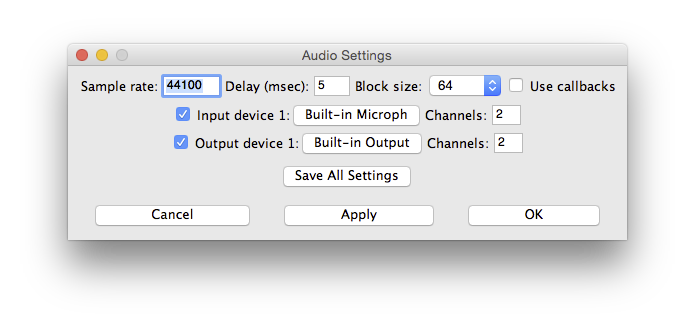
\includegraphics[scale=0.4]{fig/pd-audio.png}
    \caption{Pure Data Audio Settings}
    \label{fig:pd-audio}
\end{figure}


\begin{figure}[ht]
    \centering
    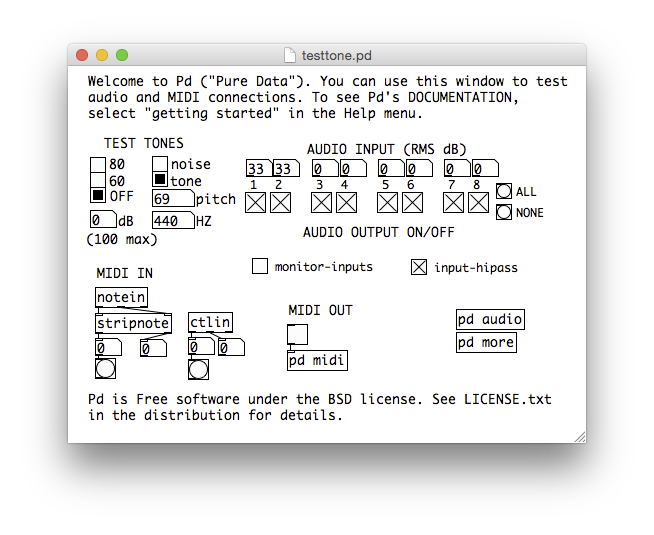
\includegraphics[scale=0.4]{fig/pd-test.png}
    \caption{Pure Data Audio Test Patch}
    \label{fig:pd-test}
\end{figure}

\begin{figure}[ht]
    \centering
    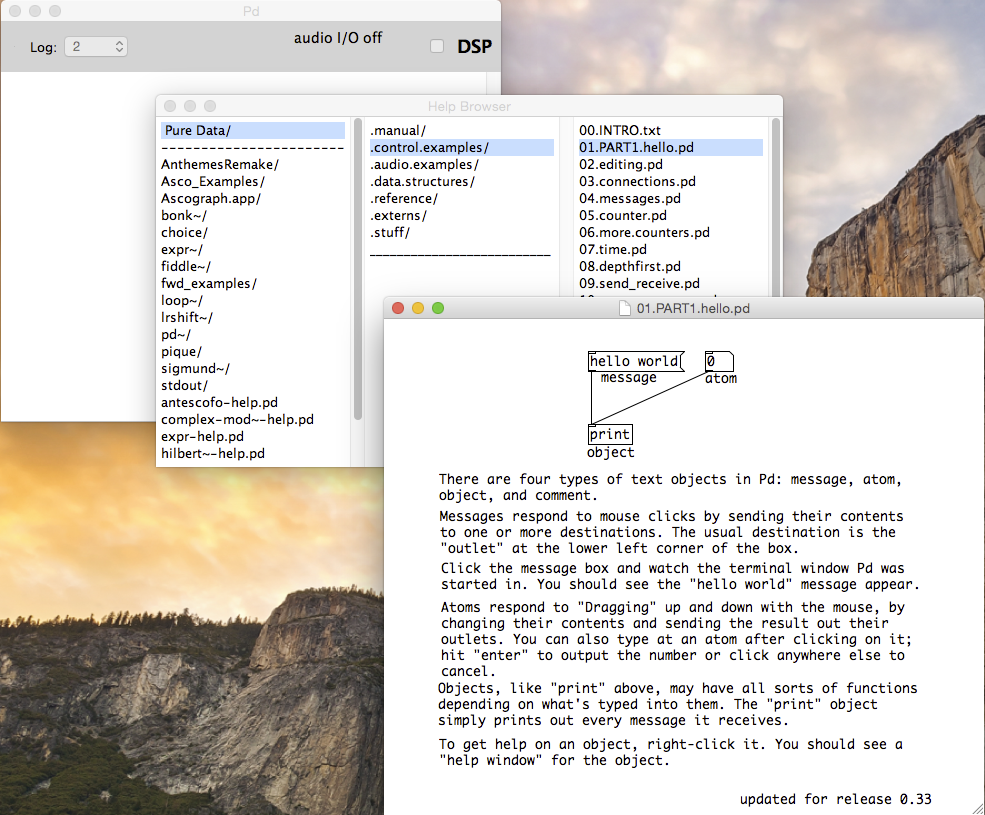
\includegraphics[scale=0.4]{fig/pd-help-browser.png}
    \caption{Pure Data Help Browser}
    \label{fig:pd-help-browser}
\end{figure}

\subsection{Implement your first Pure Data Patch}

Do something nice with Pure Data


\subsection{Getting started with Antescofo}

%audio setup. events and actions. alle meine events

Hand out the manual.

Understand events and actions.





\section{Time Table}

The time frame for the project is approximately 2 weeks, 6 hours per day, or
60 hours. Note that the time table is heavily affected by the students' prior
knowledge in programming. Table REFERENCE gives a brief overview of the
suggested time required for each individual project task.






4 weeks, preparation classes, prerequisites




\section{Acknowledgments}

The project was supported by the Austrian Research Promotion Agency (FFG) TODO: add grant number

\bibliographystyle{IEEEtran}
\bibliography{sources} 


\end{document}


